\section{Participation notes 7}
Participant: Professional

\begin{itemize}
    \item \textbf{Have them read the code-example} - Participant has no issue understanding the code. 
    \item \textbf{Have them draw the structure} - User mentions taking inspiration from DFD or Data Flow Diagram when writing. The participant then followed up by drawing the namespace as an oval and the inner functions as circles with square, triangle and a number in each. The user mentioned doing so to idenify the different functions. Under the drawing, a pipeline was drawn a square connected to the first function and then to the second function and then on to a circle. The connections were drawn as arrows. 
    \item \textbf{Have them submit the git URL} - Participant changed  the content of the repository form and used mouse to navigate once the visualization appeared. The user then mentioned that it was a good way to visualize the code.
    \item \textbf{Have them get the main() implementation} - Participant immediately clicked on the function and sees the implementation of main, but struggled to get the implementation of the other functions. 
    \item \textbf{Participant visualization} \includepdf[pages={8}]{inc/generalAppendix/userStudies/participantsVisualization.pdf}
\end{itemize}